\documentclass{standalone}
\usepackage{tikz}
\usetikzlibrary{patterns, positioning}
\usepackage[sfdefault]{ClearSans} %% option 'sfdefault' activates Clear Sans as the default text font
\usepackage[T1]{fontenc}

\begin{document}
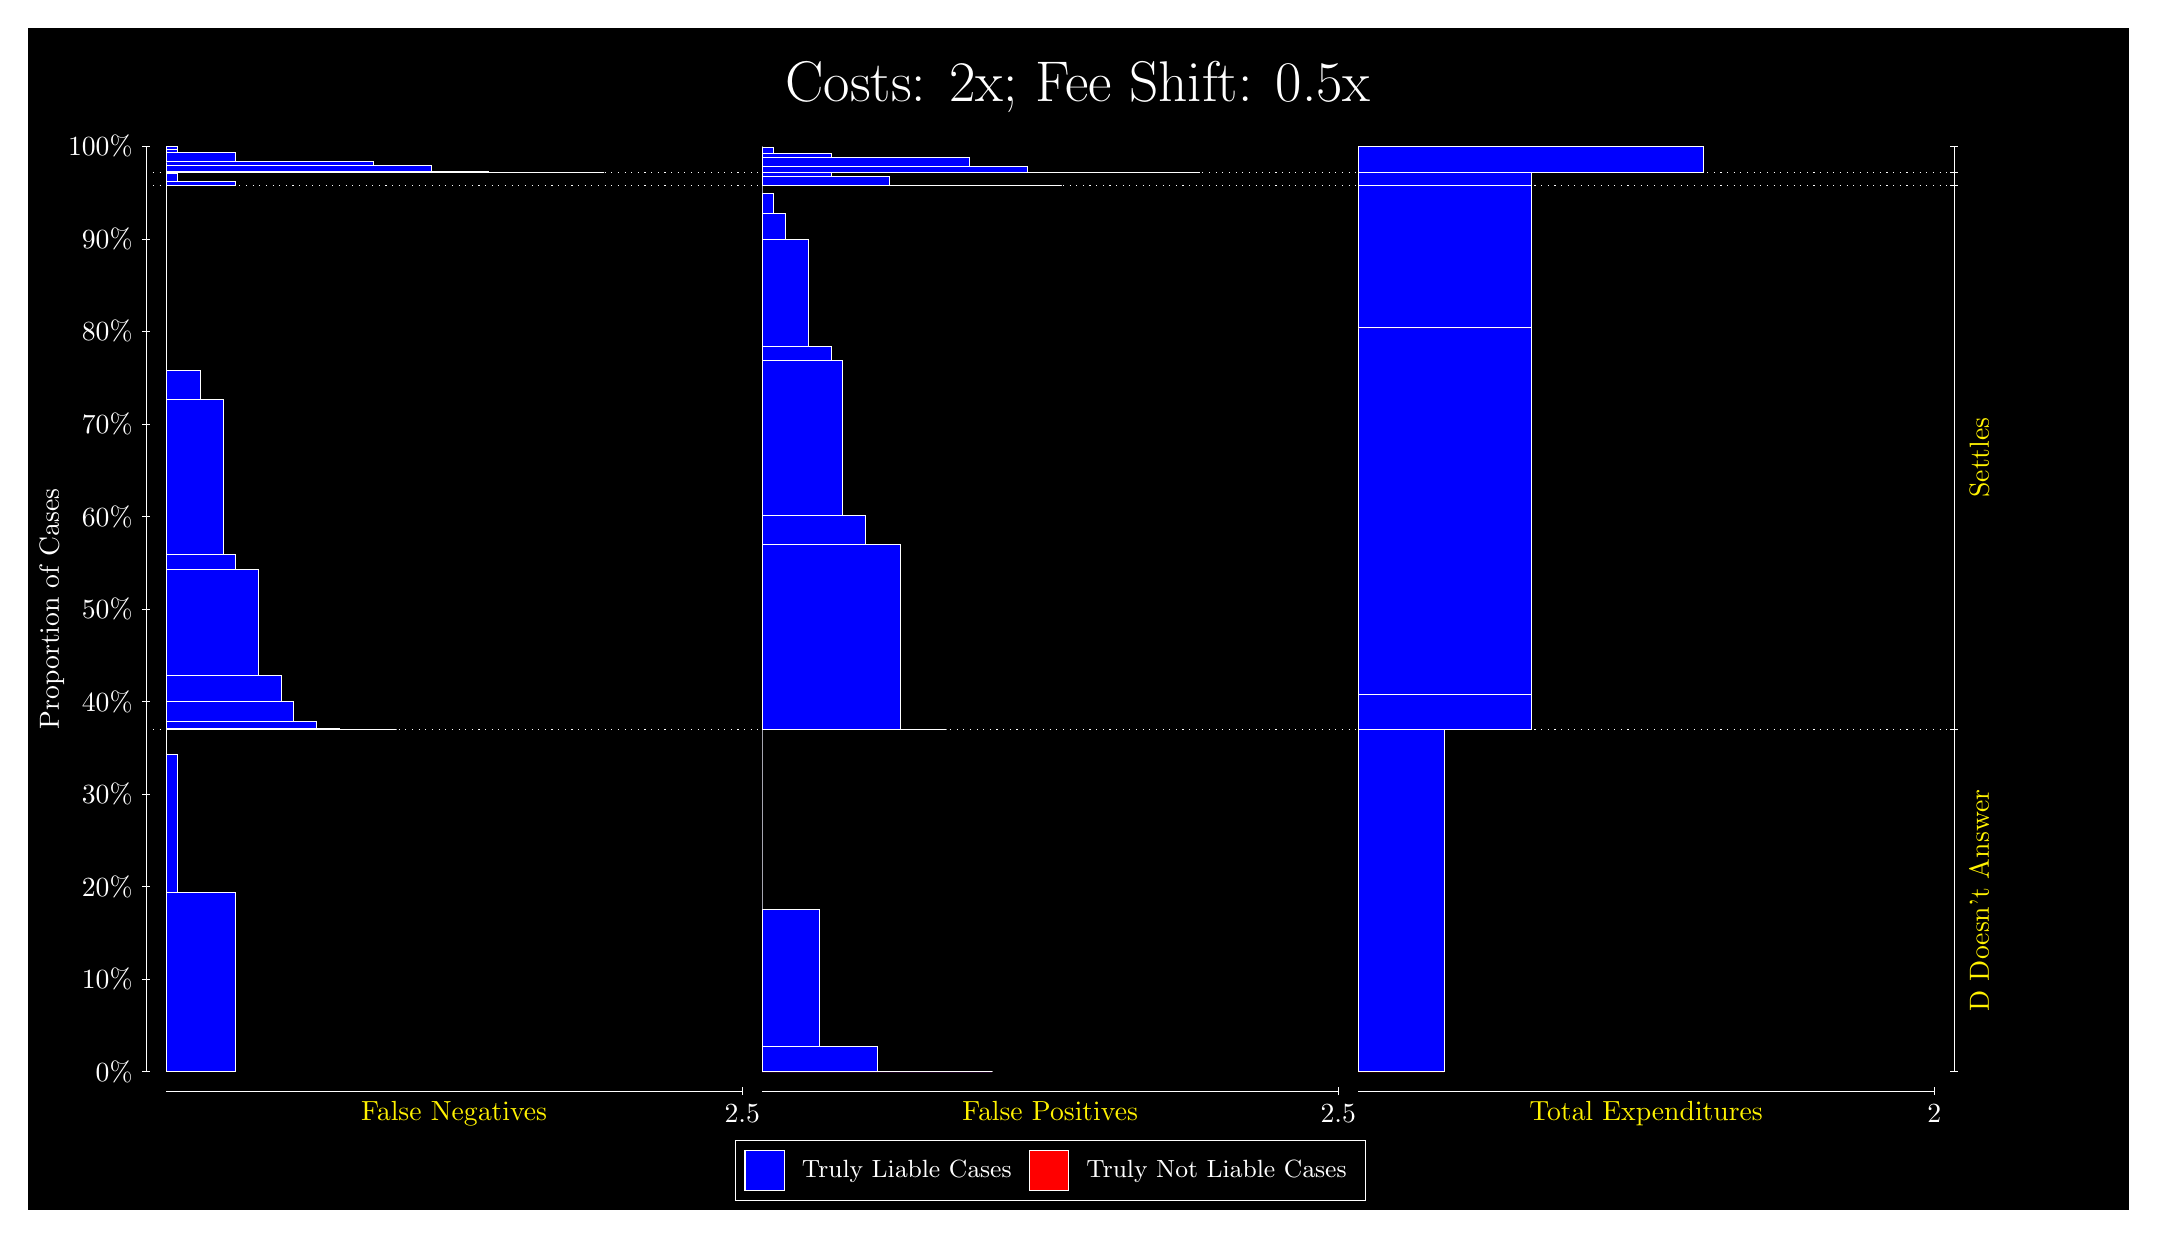
\begin{tikzpicture}
\draw[fill=black] (0,0) rectangle (26.667,15);
\draw[text=white] (0,13.5) rectangle (26.667,15) node[midway] {\huge Costs: 2x; Fee Shift: 0.5x};
\draw[white, very thin] (1.5,1.75) -- (1.5,13.5);
\node[rotate=90, text=white, anchor=center] at (0.3, 7.625) {Proportion of Cases};
\draw[white, very thin] (1.45,1.75) -- (1.55,1.75);
\node[text=white, anchor=east] at (1.45, 1.75) {0\%};
\draw[white, very thin] (1.45,2.925) -- (1.55,2.925);
\node[text=white, anchor=east] at (1.45, 2.925) {10\%};
\draw[white, very thin] (1.45,4.1) -- (1.55,4.1);
\node[text=white, anchor=east] at (1.45, 4.1) {20\%};
\draw[white, very thin] (1.45,5.275) -- (1.55,5.275);
\node[text=white, anchor=east] at (1.45, 5.275) {30\%};
\draw[white, very thin] (1.45,6.45) -- (1.55,6.45);
\node[text=white, anchor=east] at (1.45, 6.45) {40\%};
\draw[white, very thin] (1.45,7.625) -- (1.55,7.625);
\node[text=white, anchor=east] at (1.45, 7.625) {50\%};
\draw[white, very thin] (1.45,8.8) -- (1.55,8.8);
\node[text=white, anchor=east] at (1.45, 8.8) {60\%};
\draw[white, very thin] (1.45,9.975) -- (1.55,9.975);
\node[text=white, anchor=east] at (1.45, 9.975) {70\%};
\draw[white, very thin] (1.45,11.15) -- (1.55,11.15);
\node[text=white, anchor=east] at (1.45, 11.15) {80\%};
\draw[white, very thin] (1.45,12.325) -- (1.55,12.325);
\node[text=white, anchor=east] at (1.45, 12.325) {90\%};
\draw[white, very thin] (1.45,13.5) -- (1.55,13.5);
\node[text=white, anchor=east] at (1.45, 13.5) {100\%};

\draw[white, very thin] (24.457,1.75) -- (24.457,13.5);
\draw[white, very thin] (24.407,1.75) -- (24.507,1.75);
\node[anchor=west] at (24.407, 1.75) {};
\draw[white, very thin] (24.407,6.0944) -- (24.507,6.0944);
\node[anchor=west] at (24.407, 6.0944) {};
\draw[white, very thin] (24.407,13.003) -- (24.507,13.003);
\node[anchor=west] at (24.407, 13.003) {};
\draw[white, very thin] (24.407,13.171) -- (24.507,13.171);
\node[anchor=west] at (24.407, 13.171) {};
\draw[white, very thin] (24.407,13.5) -- (24.507,13.5);
\node[anchor=west] at (24.407, 13.5) {};

\draw[white, very thin, fill=blue] (1.75,1.75) rectangle (2.6283,4.0318);
\draw[white, very thin, fill=blue] (1.75,4.0318) rectangle (1.8964,5.773);
\draw[white, very thin, fill=red] (1.75,5.773) rectangle (1.75,5.773);
\draw[white, very thin, fill=blue] (1.75,5.773) rectangle (1.75,6.0944);
\draw[white, very thin, fill=blue] (1.75,6.0944) rectangle (4.6775,6.0944);
\draw[white, very thin, fill=blue] (1.75,6.0944) rectangle (4.3848,6.0945);
\draw[white, very thin, fill=blue] (1.75,6.0945) rectangle (4.092,6.1024);
\draw[white, very thin, fill=blue] (1.75,6.1024) rectangle (3.9457,6.1039);
\draw[white, very thin, fill=blue] (1.75,6.1039) rectangle (3.6529,6.197);
\draw[white, very thin, fill=blue] (1.75,6.197) rectangle (3.3602,6.4537);
\draw[white, very thin, fill=blue] (1.75,6.4537) rectangle (3.2138,6.7838);
\draw[white, very thin, fill=blue] (1.75,6.7838) rectangle (2.921,8.1313);
\draw[white, very thin, fill=blue] (1.75,8.1313) rectangle (2.6283,8.316);
\draw[white, very thin, fill=blue] (1.75,8.316) rectangle (2.4819,10.289);
\draw[white, very thin, fill=blue] (1.75,10.289) rectangle (2.1891,10.652);
\draw[white, very thin, fill=blue] (1.75,10.652) rectangle (1.8964,10.653);
\draw[white, very thin, fill=red] (1.75,10.653) rectangle (1.75,10.653);
\draw[white, very thin, fill=blue] (1.75,10.653) rectangle (1.75,13.003);
\draw[white, very thin, fill=blue] (1.75,13.003) rectangle (2.6283,13.06);
\draw[white, very thin, fill=blue] (1.75,13.06) rectangle (1.8964,13.163);
\draw[white, very thin, fill=red] (1.75,13.163) rectangle (1.75,13.163);
\draw[white, very thin, fill=blue] (1.75,13.163) rectangle (1.75,13.171);
\draw[white, very thin, fill=blue] (1.75,13.171) rectangle (7.3123,13.171);
\draw[white, very thin, fill=blue] (1.75,13.171) rectangle (6.5805,13.171);
\draw[white, very thin, fill=blue] (1.75,13.171) rectangle (5.8486,13.179);
\draw[white, very thin, fill=blue] (1.75,13.179) rectangle (5.1167,13.254);
\draw[white, very thin, fill=blue] (1.75,13.254) rectangle (4.3848,13.306);
\draw[white, very thin, fill=blue] (1.75,13.306) rectangle (4.092,13.306);
\draw[white, very thin, fill=blue] (1.75,13.306) rectangle (3.6529,13.306);
\draw[white, very thin, fill=blue] (1.75,13.306) rectangle (3.3602,13.308);
\draw[white, very thin, fill=blue] (1.75,13.308) rectangle (2.921,13.308);
\draw[white, very thin, fill=blue] (1.75,13.308) rectangle (2.6283,13.31);
\draw[white, very thin, fill=blue] (1.75,13.31) rectangle (2.6283,13.421);
\draw[white, very thin, fill=blue] (1.75,13.421) rectangle (1.8964,13.457);
\draw[white, very thin, fill=blue] (1.75,13.457) rectangle (1.8964,13.496);
\draw[white, very thin, fill=red] (1.75,13.496) rectangle (1.75,13.496);
\draw[white, very thin, fill=blue] (1.75,13.496) rectangle (1.75,13.5);
\draw[white, very thin, fill=red] (9.3189,1.75) rectangle (12.246,1.75);
\draw[white, very thin, fill=blue] (9.3189,1.75) rectangle (12.246,1.75);
\draw[white, very thin, fill=blue] (9.3189,1.75) rectangle (11.515,1.7527);
\draw[white, very thin, fill=blue] (9.3189,1.7527) rectangle (10.783,2.0714);
\draw[white, very thin, fill=blue] (9.3189,2.0714) rectangle (10.051,3.8127);
\draw[white, very thin, fill=blue] (9.3189,3.8127) rectangle (9.3189,6.0944);
\draw[white, very thin, fill=red] (9.3189,6.0944) rectangle (11.661,6.0944);
\draw[white, very thin, fill=blue] (9.3189,6.0944) rectangle (11.661,6.0944);
\draw[white, very thin, fill=red] (9.3189,6.0944) rectangle (11.368,6.0944);
\draw[white, very thin, fill=blue] (9.3189,6.0944) rectangle (11.368,6.0981);
\draw[white, very thin, fill=red] (9.3189,6.0981) rectangle (11.075,6.0981);
\draw[white, very thin, fill=blue] (9.3189,6.0981) rectangle (11.075,8.4443);
\draw[white, very thin, fill=blue] (9.3189,8.4443) rectangle (10.929,8.446);
\draw[white, very thin, fill=blue] (9.3189,8.446) rectangle (10.636,8.8086);
\draw[white, very thin, fill=blue] (9.3189,8.8086) rectangle (10.344,10.782);
\draw[white, very thin, fill=blue] (9.3189,10.782) rectangle (10.197,10.966);
\draw[white, very thin, fill=blue] (9.3189,10.966) rectangle (9.9044,12.314);
\draw[white, very thin, fill=blue] (9.3189,12.314) rectangle (9.6116,12.644);
\draw[white, very thin, fill=blue] (9.3189,12.644) rectangle (9.4652,12.901);
\draw[white, very thin, fill=blue] (9.3189,12.901) rectangle (9.3189,13.003);
\draw[white, very thin, fill=red] (9.3189,13.003) rectangle (13.125,13.003);
\draw[white, very thin, fill=blue] (9.3189,13.003) rectangle (13.125,13.003);
\draw[white, very thin, fill=blue] (9.3189,13.003) rectangle (12.393,13.003);
\draw[white, very thin, fill=blue] (9.3189,13.003) rectangle (11.661,13.011);
\draw[white, very thin, fill=blue] (9.3189,13.011) rectangle (10.929,13.115);
\draw[white, very thin, fill=blue] (9.3189,13.115) rectangle (10.197,13.171);
\draw[white, very thin, fill=red] (9.3189,13.171) rectangle (14.881,13.171);
\draw[white, very thin, fill=blue] (9.3189,13.171) rectangle (14.881,13.171);
\draw[white, very thin, fill=red] (9.3189,13.171) rectangle (14.149,13.171);
\draw[white, very thin, fill=blue] (9.3189,13.171) rectangle (14.149,13.171);
\draw[white, very thin, fill=red] (9.3189,13.171) rectangle (13.417,13.171);
\draw[white, very thin, fill=blue] (9.3189,13.171) rectangle (13.417,13.175);
\draw[white, very thin, fill=blue] (9.3189,13.175) rectangle (12.686,13.251);
\draw[white, very thin, fill=blue] (9.3189,13.251) rectangle (11.954,13.363);
\draw[white, very thin, fill=red] (9.3189,13.363) rectangle (11.661,13.363);
\draw[white, very thin, fill=blue] (9.3189,13.363) rectangle (11.661,13.363);
\draw[white, very thin, fill=blue] (9.3189,13.363) rectangle (11.222,13.365);
\draw[white, very thin, fill=red] (9.3189,13.365) rectangle (10.929,13.365);
\draw[white, very thin, fill=blue] (9.3189,13.365) rectangle (10.929,13.365);
\draw[white, very thin, fill=blue] (9.3189,13.365) rectangle (10.49,13.365);
\draw[white, very thin, fill=blue] (9.3189,13.365) rectangle (10.197,13.418);
\draw[white, very thin, fill=red] (9.3189,13.418) rectangle (10.197,13.418);
\draw[white, very thin, fill=blue] (9.3189,13.418) rectangle (10.197,13.418);
\draw[white, very thin, fill=blue] (9.3189,13.418) rectangle (9.4652,13.49);
\draw[white, very thin, fill=blue] (9.3189,13.49) rectangle (9.4652,13.493);
\draw[white, very thin, fill=blue] (9.3189,13.493) rectangle (9.3189,13.5);
\draw[white, very thin, fill=red] (16.888,1.75) rectangle (17.986,1.75);
\draw[white, very thin, fill=blue] (16.888,1.75) rectangle (17.986,6.0944);
\draw[white, very thin, fill=red] (16.888,6.0944) rectangle (19.083,6.0944);
\draw[white, very thin, fill=blue] (16.888,6.0944) rectangle (19.083,6.5454);
\draw[white, very thin, fill=red] (16.888,6.5454) rectangle (19.083,6.5454);
\draw[white, very thin, fill=blue] (16.888,6.5454) rectangle (19.083,11.196);
\draw[white, very thin, fill=red] (16.888,11.196) rectangle (19.083,11.196);
\draw[white, very thin, fill=blue] (16.888,11.196) rectangle (19.083,13.003);
\draw[white, very thin, fill=red] (16.888,13.003) rectangle (19.083,13.003);
\draw[white, very thin, fill=blue] (16.888,13.003) rectangle (19.083,13.171);
\draw[white, very thin, fill=red] (16.888,13.171) rectangle (21.279,13.171);
\draw[white, very thin, fill=blue] (16.888,13.171) rectangle (21.279,13.5);
\draw[white, dotted] (1.5,6.0944) -- (24.457,6.0944);
\draw[white, dotted] (1.5,13.003) -- (24.457,13.003);
\draw[white, dotted] (1.5,13.171) -- (24.457,13.171);
\draw[white, very thin] (1.75,1.5) -- (9.0689,1.5);
\node[text=yellow, anchor=north] at (5.4094, 1.5) {False Negatives};
\draw[white, very thin] (9.0689,1.45) -- (9.0689,1.55);
\node[text=white, anchor=north] at (9.0689, 1.45) {2.5};

\draw[white, very thin] (9.3189,1.5) -- (16.638,1.5);
\node[text=yellow, anchor=north] at (12.978, 1.5) {False Positives};
\draw[white, very thin] (16.638,1.45) -- (16.638,1.55);
\node[text=white, anchor=north] at (16.638, 1.45) {2.5};

\draw[white, very thin] (16.888,1.5) -- (24.207,1.5);
\node[text=yellow, anchor=north] at (20.547, 1.5) {Total Expenditures};
\draw[white, very thin] (24.207,1.45) -- (24.207,1.55);
\node[text=white, anchor=north] at (24.207, 1.45) {2};

\node[text=yellow, centered, rotate=90] at (24.777, 3.9222) {D Doesn't Answer};
\node[text=yellow, centered, rotate=90] at (24.777, 9.5488) {Settles};



\draw (12.978300999999998,1.5) node[draw=none] (baseCoordinate) {};
\begin{scope}[align=center]
        \matrix[scale=0.5, draw=white, below=0.5cm of baseCoordinate, nodes={draw}, column sep=0.1cm]{
            \node[rectangle, draw, minimum width=0.5cm, minimum height=0.5cm, fill=blue] {}; &
            \node[draw=none, font=\small, text=white] (B) {Truly Liable Cases}; &
            \node[rectangle, draw, minimum width=0.5cm, minimum height=0.5cm, fill=red] {}; &
            \node[draw=none, font=\small, text=white] (B) {Truly Not Liable Cases}; \\
            };
\end{scope}

\end{tikzpicture}
\end{document}